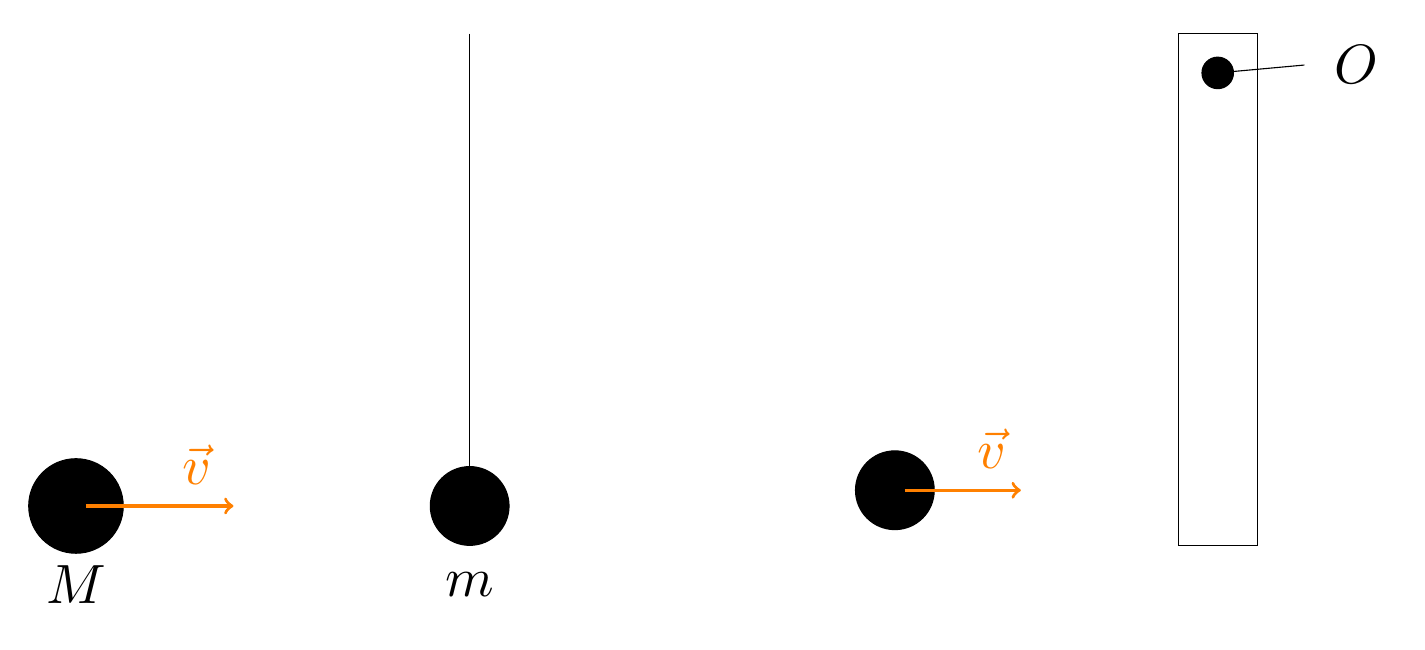
\begin{tikzpicture}

\draw  (2,3) rectangle (3,-3.5);

\draw (-7,3) -- (-7,-3) node (v1) {};
\draw  [fill] (v1) circle (0.5);
\draw  [fill] (-1.6,-2.8) node (v2) {} circle (0.5);
\draw  [fill] (2.5,2.5) node (v4) {} circle (0.2);
\draw  [fill] (-12,-3) node (v3) {} circle (0.6);
\draw [->,very thick, orange] (v2) -- (0,-2.8) node [near end, above, scale=2, orange]{$\vec{v}$};
\draw [->,very thick,orange] (v3) -- (-10,-3) node [near end, above, scale=2, orange]{$\vec{v}$};
\draw (v4) -- (3.6,2.6) node [scale=2, right=2]{$O$};
\node at (-12,-4) [scale=2]{$M$};
\node at (-7,-4) [scale=2]{$m$};
\end{tikzpicture}